\chapter{随机抽样}
\section{Monte Carlo方法}
Monte Carlo方法是用随机数解决计算问题方法的统称。
\begin{method}{von Neumann舍选法}{}
	\begin{enumerate}
		\item 选取容易抽样的分布$h(x)$，使得曲线$Ch(x)$可以覆盖待抽样的分布$f(x)$；
		\item 从$h(x)$抽样得$x_i$；
		\item 从$\UnifDist(0,1)$抽样得$r_i$；
		\item 若$r_iCh(x_i)\leqslant f(x_i)$，则保留$x_i$，否则舍弃；
		\item 被接受的$x_i$序列，服从以$f(x)$为概率密度的分布；
		\item 使用$x_i$序列的算术平均，估算数学期望
	\end{enumerate}
	\begin{notecaptionblock}
		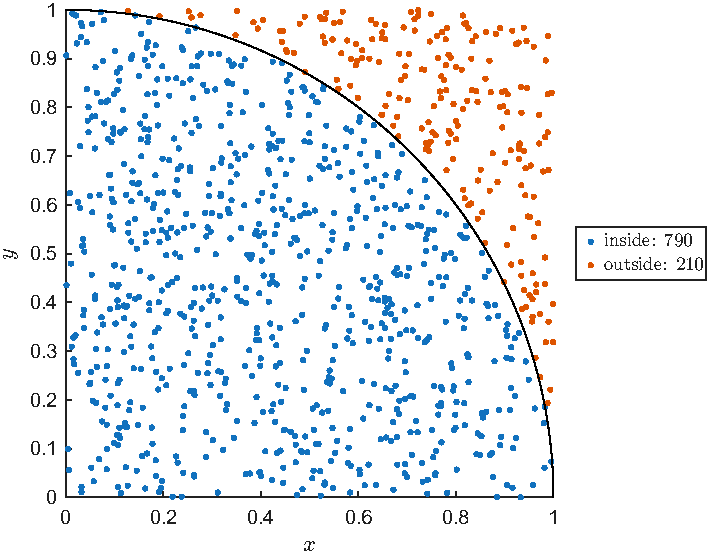
\includegraphics[width=0.6\linewidth]{figures/monte_carlo.pdf}
		\captionof{figure}{von Neumann舍选法计算$\pi\approx 4\times\frac{790}{1000}=3.16$}
		\label{fig:monte_carlo}
	\end{notecaptionblock}
\end{method}

\noindent
舍选法也适用于仅知比例的目标密度，只要能给出覆盖该未归一化密度的包络。

\begin{method}{Markov链法}{}
	设$f$与目标密度成正比。在当前点$x$按提议密度$q(y\mid x)$生成候选$y$，以概率
	\[
		\min\biggb{1,\frac{f(y)q(x\mid y)}{f(x)q(y\mid x)}}
	\]
	接受$y$，否则保留$x$。这个转移核对目标分布满足细致平衡。若提议对称，接受比简化为$f(y)/f(x)$。由任意起点抽样还需检查链的遍历性。
\end{method}

\section{Bootstrap自助法}

\begin{quote}
	\textit{Why can not a man lift himself by pulling up on his bootstraps?}
\end{quote}
\begin{method}{bootstrap自助法}{}
	\begin{compactenum}
		\item 把样本看作总体的估计
		\item 从样本抽样(可放回)，得到bootstrap样本
		\item 计算bootstrap样本的统计量
	\end{compactenum}
	\begin{notecaptionblock}
		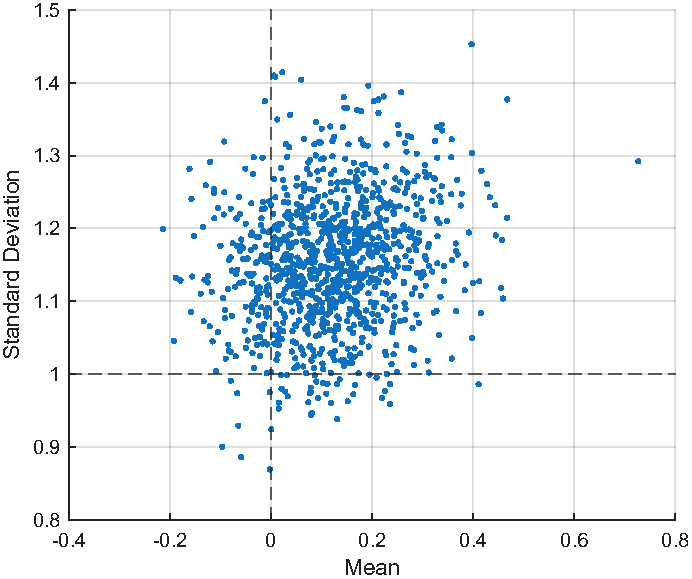
\includegraphics[width=0.6\linewidth]{figures/bootstrap.pdf}
		\captionof{figure}{对标准正态分布$\NormalDist(0,1)$的100个样本进行1000次bootstrap自助法得到的样本均值和方差分布}
		\label{fig:bootstrap}
	\end{notecaptionblock}
\end{method}
\begin{definition}{经验分布函数}{}
	$x_1,\ldots,x_n$是来自分布函数为$\CDF(x)$总体$X$的样本观察值。$X$的经验分布函数$\CDF_n(x)$定义为
	\begin{equation}
		\CDF_n(x)=\frac1n\sum_{i=1}^nI(x\geqslant x_i).
	\end{equation}
	用经验分布函数$\CDF_n$估计总体分布函数$\CDF$。
\end{definition}
从$\CDF_n$抽样可以看作是对样本$x_1,\ldots,x_n$进行可放回的重新抽样，称作bootstrap样本，记为$x_1^\ast,\ldots,$或$\bm x^\ast$。

使用一系列$\bm x^\ast$，得到相应的$\hat\theta_b^\ast=\hat\theta(\bm x_b^\ast)$。定义
\[
	\avg\theta^\ast=\frac1B\sum_{b=1}^B\hat\theta_b^\ast.
\]
它估计给定样本时的重抽样期望$\E_\ast(\hat\theta^\ast)$。$\avg\theta^\ast-\hat\theta$用于估计原统计量的偏差。

\begin{theorem}{样本均值的bootstrap中心极限定理}{bootstrap CLT}
	若原样本独立同分布，均值为$\mu$，方差为$0<\sigma^2<\infty$，记$\P_\ast$为给定样本的重抽样概率。对每个实数$t$，
	\begin{equation}
		\P_\ast\bigp{\sqrt n(\avg X^\ast-\avg X)\le t}
		\pto\Phi(t/\sigma).
	\end{equation}
	因此条件重抽样分布和$\sqrt n(\avg X-\mu)$的抽样分布具有相同的正态极限。更高阶精度需要额外的光滑性、矩条件以及合适的统计量。
\end{theorem}
